\documentclass[pdftex,12pt,a4paper]{article}
\newcommand{\HRule}{\rule{\linewidth}{0.5mm}}
\linespread{1.3}
\usepackage{graphicx}
\usepackage[margin=2.75cm]{geometry}
\usepackage{tikz}
\usepackage{amsmath}
\usepackage{hyperref}
\usepackage{algorithm}
 \usepackage{algpseudocode}
\usetikzlibrary{decorations.pathmorphing}
\usetikzlibrary{shapes}
\tikzset{snake it/.style={decorate, decoration=snake}}


\begin{document}



%%%%%%%%%%%%%%%%%%%%%%
%%%%% TITLE PAGE %%%%%
%%%%%%%%%%%%%%%%%%%%%%

\begin{titlepage}
\begin{center}
\pagenumbering{gobble}

\begin{figure}

\centering
\includegraphics[width=30mm]{Crest.png}

\end{figure}


\textsc{\LARGE Trinity College Dublin}\\
\textsc{\Large School of Mathematics}

\HRule \\[0.4cm]
{\huge \bfseries Spin models on random bipartite graphs \\[0.4cm] }

\HRule \\[1.5cm]

\Large \emph{Author:} \\ Shane Harding \\[0.8cm]

\large \emph{Supervisor:} \\ Prof. Mike Peardon

\end{center}

\end{titlepage}

%%%%%%%%%%%%%%%%%%%%%%



\pagenumbering{roman}
%%%%%%%%%%%%%%%%%%%%
%%%%% ABSTRACT %%%%%
%%%%%%%%%%%%%%%%%%%%

\vspace*{\fill}
\begin{abstract}

This is my abstract.

\end{abstract}
\vspace*{\fill}

\newpage

%%%%%%%%%%%%%%%%%%%%%%%%%%%%%
%%%%% TABLE OF CONTENTS %%%%%
%%%%%%%%%%%%%%%%%%%%%%%%%%%%%

\tableofcontents

\newpage
\pagenumbering{arabic}


%%%%%%%%%%%%%%%%%%%%%%%%
%%%%% INTRODUCTION %%%%%
%%%%%%%%%%%%%%%%%%%%%%%%

\section{Introduction}

This project is centered around doing Ising Model simulations on random bipartite graphs. As such, it is useful to know more the Ising model and graph theory before we get started.

%%%%% ISING MODEL %%%%%

\subsection{The Ising Model}

\subsubsection{What is the Ising Model?}

The Ising Model is a mathematical model that was invented by Wilhelm Lenz, but developed by Ernst Ising in 1925. It is used to to explore ferromagnetism in statistical physics.

\subsubsection{Analytical tools used for studying the Ising Model}

\subsubsection{How it is normally studied in serial and parallel simulations}

The two dimenstional Ising model is usually represented as a rectangular lattice, sometimes with periodic boundary conditions and sometimes not, depending on the case in question. Each point on the lattice is assigned a spin at the start of the simulation, usually at random. Each point only `feels' the interaction of its nearest neighbours (each point has four neighbours). These interactions allow a Hamiltonian to be calculated for each point.

FILL ABOUT METROPOLIS HASTINGS AND UPDATING POINTS

In parallel we divide the grid up into smaller subgrids. In the figure, the grid is divided into four subgrids but obviously more subdivisions are possible. Normally we have one subgrid per processor that we intend to run the program on. The need for \emph{Message Passing Interface} (MPI) function calls arises from the fact that on the edges of our subgrids there are points needed for the update step whose values are stored on another processor. These values need to be identified and passed to the relevant processor. MPI is used for this task.

%%%%% REGULAR LATTICE ISING PIC %%%%%
\begin{figure}
\begin{center}
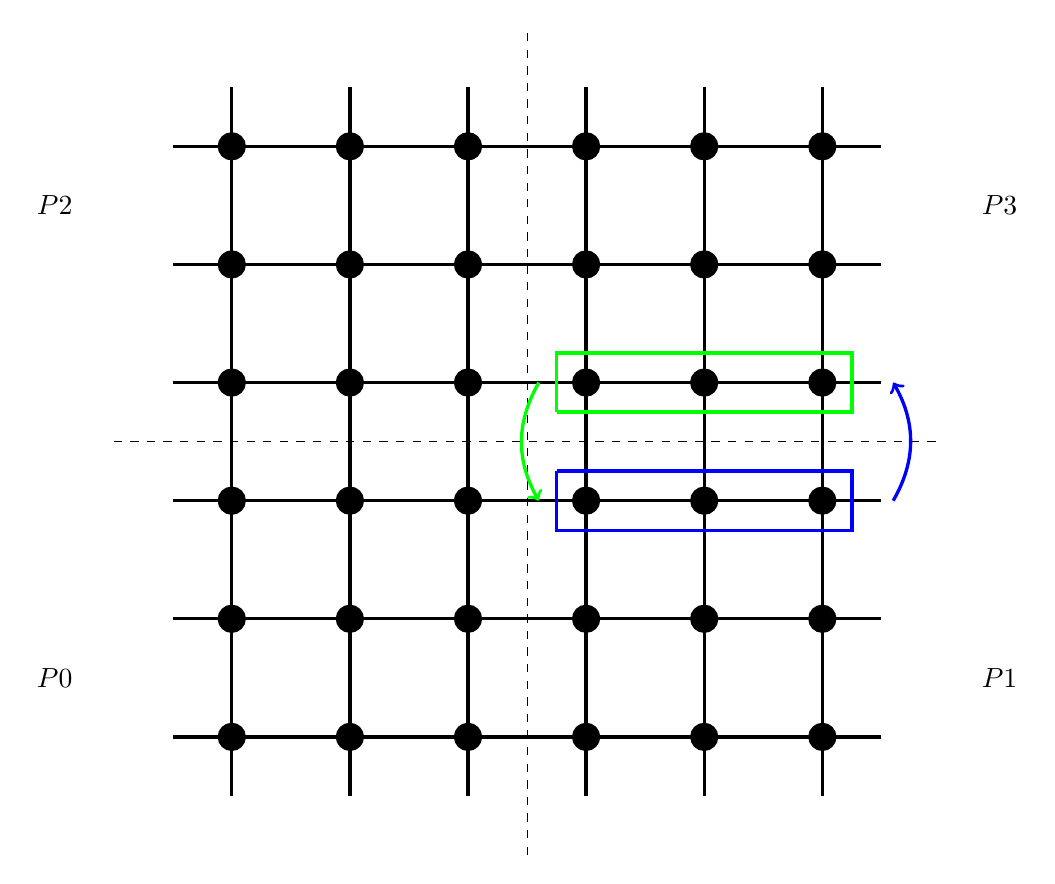
\begin{tikzpicture}[scale=1.5]

\node at (-4, -2) {$P0$};
\node at (4,-2) {$P1$};
\node at (-4, 2) {$P2$};
\node at (4,2) {$P3$};

\draw [very thick] (-3,-2.5) -- (3,-2.5);
\draw [very thick] (-3,-1.5) -- (3,-1.5);
\draw [very thick] (-3,-0.5) -- (3,-0.5);
\draw [very thick] (-3,0.5) -- (3,0.5);
\draw [very thick] (-3,1.5) -- (3,1.5);
\draw [very thick] (-3,2.5) -- (3,2.5);

\draw [dashed] (-3.5,0) -- (3.5,0);
\draw [dashed] (0,-3.5) -- (0,3.5);

\draw [very thick] (-2.5,-3) -- (-2.5,3);
\draw [very thick] (-1.5,-3) -- (-1.5,3);
\draw [very thick] (-0.5,-3) -- (-0.5,3);
\draw [very thick] (0.5,-3) -- (0.5,3);
\draw [very thick] (1.5,-3) -- (1.5,3);
\draw [very thick] (2.5,-3) -- (2.5,3);

\draw [blue,very thick] (0.25, -0.25) -- (0.25, -0.75) -- (2.75,-0.75) -- (2.75,-0.25) -- (0.25, -0.25);
\draw [->][blue, very thick] (3.1,-0.5) to [out=60,in=300] (3.1,0.5);

\draw [green,very thick] (0.25, 0.25) -- (0.25, 0.75) -- (2.75,0.75) -- (2.75,0.25) -- (0.25, 0.25);
\draw [->][green, very thick] (0.1,0.5) to [out=240,in=120] (0.1,-0.5);

\draw [fill=black,very thick] (-2.5,-2.5) circle (3pt);
\draw [fill=black,very thick] (-1.5,-2.5) circle (3pt);
\draw [fill=black,very thick] (-0.5,-2.5) circle (3pt);
\draw [fill=black,very thick] (0.5,-2.5) circle (3pt);
\draw [fill=black,very thick] (1.5,-2.5) circle (3pt);
\draw [fill=black,very thick] (2.5,-2.5) circle (3pt);

\draw [fill=black,very thick] (-2.5,-1.5) circle (3pt);
\draw [fill=black,very thick] (-1.5,-1.5) circle (3pt);
\draw [fill=black,very thick] (-0.5,-1.5) circle (3pt);
\draw [fill=black,very thick] (0.5,-1.5) circle (3pt);
\draw [fill=black,very thick] (1.5,-1.5) circle (3pt);
\draw [fill=black,very thick] (2.5,-1.5) circle (3pt);

\draw [fill=black,very thick] (-2.5,-0.5) circle (3pt);
\draw [fill=black,very thick] (-1.5,-0.5) circle (3pt);
\draw [fill=black,very thick] (-0.5,-0.5) circle (3pt);
\draw [fill=black,very thick] (0.5,-0.5) circle (3pt);
\draw [fill=black,very thick] (1.5,-0.5) circle (3pt);
\draw [fill=black,very thick] (2.5,-0.5) circle (3pt);

\draw [fill=black,very thick] (-2.5,0.5) circle (3pt);
\draw [fill=black,very thick] (-1.5,0.5) circle (3pt);
\draw [fill=black,very thick] (-0.5,0.5) circle (3pt);
\draw [fill=black,very thick] (0.5,0.5) circle (3pt);
\draw [fill=black,very thick] (1.5,0.5) circle (3pt);
\draw [fill=black,very thick] (2.5,0.5) circle (3pt);

\draw [fill=black,very thick] (-2.5,1.5) circle (3pt);
\draw [fill=black,very thick] (-1.5,1.5) circle (3pt);
\draw [fill=black,very thick] (-0.5,1.5) circle (3pt);
\draw [fill=black,very thick] (0.5,1.5) circle (3pt);
\draw [fill=black,very thick] (1.5,1.5) circle (3pt);
\draw [fill=black,very thick] (2.5,1.5) circle (3pt);

\draw [fill=black,very thick] (-2.5,2.5) circle (3pt);
\draw [fill=black,very thick] (-1.5,2.5) circle (3pt);
\draw [fill=black,very thick] (-0.5,2.5) circle (3pt);
\draw [fill=black,very thick] (0.5,2.5) circle (3pt);
\draw [fill=black,very thick] (1.5,2.5) circle (3pt);
\draw [fill=black,very thick] (2.5,2.5) circle (3pt);

\end{tikzpicture}
\caption{Regular square lattice Ising model.}
\end{center}
\end{figure}

%%%%% GRAPH THEORY %%%%%

\subsection{Graph Theory}

Graph theory refers to the mathematical study of \emph{graphs}. A graph is a visual representation of set of objects, known as \emph{vertices}. Some pairs of these obects are then connected by links, known as \emph{edges}. If the edges are said to have orientation (if edge $(a, b) \neq (b, a)$, where $a, b$ are vertices), then we call the graph a directed graph. If the edges don't have orientation (if $(a,b)=(b,a)$) then we call the graph an undirected graph. We will deal only with undirected graphs in this report.

For this project we're not going to consider disconnected graphs. That is, graphs where there are no nodes connecting a vertex, or set of connected vertices, to the rest of the graph. Only connected graphs are considered.

All graphs considered will be random, \emph{bipartite} graphs. A bipartite graph is a graph in which we can divide its vertices into two disjoint sets, $A$ and $B$, such that vertices in $A$ are only connected to vertices in $B$, and vice versa. Disjoint means that the two sets have no element in common.

A random graph is a graph where the edges connect vertices at random; there is no pattern or order to how vertices are connected.

\emph{Trivalent graphs} are another class of the graphs we will be dealing with a lot. For a graph to be trivalent it means that ever vertex has exactly three edges connecting it to three other distinct vertices.

\begin{figure}
\begin{center}
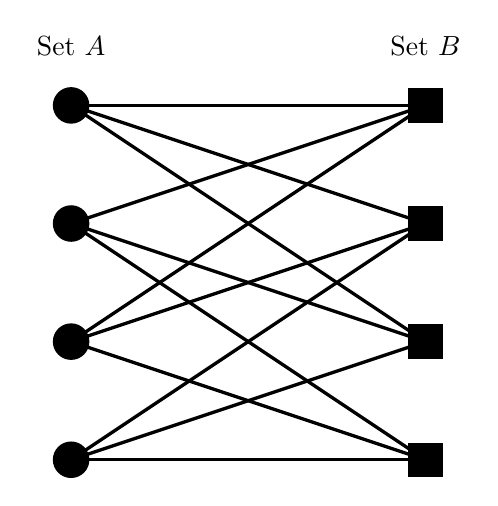
\begin{tikzpicture}[scale=1.5]

\node at (-1.5, 2) {Set $A$};
\node at (1.5, 2) {Set $B$};

\draw [fill=black,very thick] (-1.5,1.5) circle (4pt);
\draw [fill=black,very thick] (-1.5,0.5) circle (4pt);
\draw [fill=black,very thick] (-1.5,-0.5) circle (4pt);
\draw [fill=black,very thick] (-1.5,-1.5) circle (4pt);

\filldraw ([xshift=-4pt,yshift=-4pt]1.5,1.5) rectangle ++(8pt,8pt);
\filldraw ([xshift=-4pt,yshift=-4pt]1.5,0.5) rectangle ++(8pt,8pt);
\filldraw ([xshift=-4pt,yshift=-4pt]1.5,-0.5) rectangle ++(8pt,8pt);
\filldraw ([xshift=-4pt,yshift=-4pt]1.5,-1.5) rectangle ++(8pt,8pt);

\draw [very thick] (-1.5,1.5) -- (1.5,1.5);
\draw [very thick] (-1.5,1.5) -- (1.5,0.5);
\draw [very thick] (-1.5,1.5) -- (1.5,-0.5);

\draw [very thick] (-1.5,0.5) -- (1.5,-1.5);
\draw [very thick] (-1.5,0.5) -- (1.5,-0.5);
\draw [very thick] (-1.5,0.5) -- (1.5,1.5);

\draw [very thick] (-1.5,-0.5) -- (1.5,1.5);
\draw [very thick] (-1.5,-0.5) -- (1.5,-1.5);
\draw [very thick] (-1.5,-0.5) -- (1.5,0.5);

\draw [very thick] (-1.5,-1.5) -- (1.5,-0.5);
\draw [very thick] (-1.5,-1.5) -- (1.5,-1.5);
\draw [very thick] (-1.5,-1.5) -- (1.5,0.5);


\end{tikzpicture}
\caption{A random bipartite trivalent graph.}
\end{center}
\end{figure}

%%%%% MOTIVATION %%%%%

\subsection{Motivation}

%%%%% MPI %%%%%

\subsubsection{Why this is an interesting MPI problem}

%%%%% PHYSICS %%%%%

\subsubsection{Physical uses of these simulations}


%%%%% AIMS %%%%%
\subsection{Aims}

\newpage
%%%%%%%%%%%%%%%%%%%%%%%%%%%%%%%%%
%%%%% SOFTWARE ARCHITECTURE %%%%%
%%%%%%%%%%%%%%%%%%%%%%%%%%%%%%%%%

\section{Software Architecture}

In this section I will discuss the various techniques used in creating the simulations that were run in the duration of this project. The main areas these fall under are: graph generating - in both serial and parallel, as well as associated swap algorithms; MPI communication structure; and, finally, how the update step worked.

\subsection{Random graph generation}

Over the course of this project numerous different methods were implemented and compared for the `best' way to create a random bipartite graph. These methods were written in both serial and parallel.

%%%%% RANDOM GRAPHS %%%%%
\subsubsection{Generating random graphs in serial}

%%%%% SWAP ALG %%%%%
\subsubsection{Swap algorithms in serial and parallel}

The swap aglorithm is used for two purposes in this project. The first in the generation of random graphs, and the second is as a proposal step during an update (instead of proposing a spin flip a swap is proposed instead. The reasoning and implementation of both of this will be addressed in a while but first we will look at how the swap alogrithm works.

\paragraph{The algorithm} ~\\

The algorithm works by first choosing a node in set $A$, at random, which we will call $a_0$ . From this node two of its neighbours in set $B$ are chosen (again, at random), we call these $b_1$ and $b_2$. The next step is to choose one neighbour each of $b_1$ and $b_2$, ensuring not to choose $a_0$ again. Label the neighbour of $b_1$ as $a_1$ and the neighbour of $b_2$ as $a_2$. At this point we have the nodes selected that we wish to swap. We want to have $b_1$ not connected to $a_1$ anymore, but instead have it connected to $a_2$, and similarly no longer have $b_2$ connected to $a_2$, but connected to $a_1$.

Before we can do this however we must preform some checks. We must ensure that $a_1$ is not connected to $b_2$ by any other edge that we have not considered so far, and similarly we must must ensure that $a_2$ is in no way connected to $b_1$. The reason for this check is that we may already have the nodes we wish to swap connected to each other by another edge, so if the swap is performed then it would mean having two edges connecting the same two points to each other, which is not desirable.

%%%%% SWAP ALG PIC %%%%%
\begin{figure}
\begin{center}
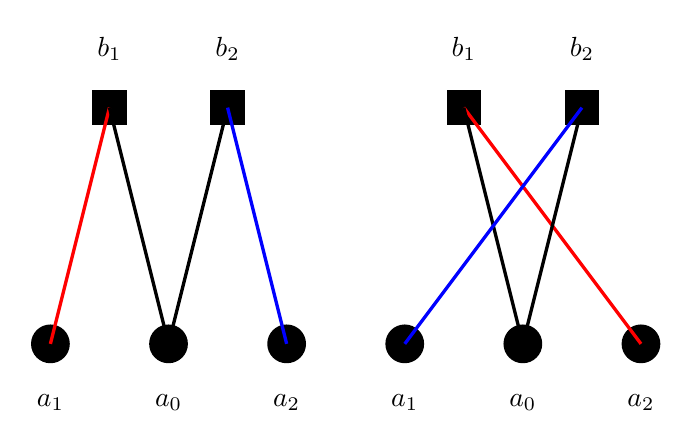
\begin{tikzpicture}[scale=1.5]

\draw [fill=black,very thick] (-2.5,-1) circle (0.15cm);
\node at (-2.5, -1.5) {$a_1$};
\draw [fill=black,very thick] (-1.5,-1) circle (0.15cm);
\node at (-1.5, -1.5) {$a_0$};
\draw [fill=black,very thick] (-0.5,-1) circle (0.15cm);
\node at (-0.5, -1.5) {$a_2$};

\filldraw ([xshift=-4pt,yshift=-4pt] -2,1) rectangle ++(8pt,8pt);
\node at (-2, 1.5) {$b_1$};
\filldraw ([xshift=-4pt,yshift=-4pt] -1,1) rectangle ++(8pt,8pt);
\node at (-1, 1.5) {$b_2$};

\draw [red, very thick] (-2.5,-1) -- (-2,1);
\draw [very thick] (-2,1) -- (-1.5,-1);
\draw [very thick] (-1.5,-1) -- (-1,1);
\draw [blue, very thick] (-1,1) -- (-0.5,-1);

\draw [fill=black,very thick] (2.5,-1) circle (0.15cm);
\node at (2.5, -1.5) {$a_2$};
\draw [fill=black,very thick] (1.5,-1) circle (0.15cm);
\node at (1.5, -1.5) {$a_0$};
\draw [fill=black,very thick] (0.5,-1) circle (0.15cm);
\node at (0.5, -1.5) {$a_1$};

\filldraw ([xshift=-4pt,yshift=-4pt] 2,1) rectangle ++(8pt,8pt);
\node at (2, 1.5) {$b_2$};
\filldraw ([xshift=-4pt,yshift=-4pt] 1,1) rectangle ++(8pt,8pt);
\node at (1, 1.5) {$b_1$};

\draw [red, very thick] (2.5,-1) -- (1,1);
\draw [very thick] (2,1) -- (1.5,-1);
\draw [very thick] (1.5,-1) -- (1,1);
\draw [blue, very thick] (0.5,-1) -- (2,1);

\end{tikzpicture}
\caption{Swap alg.}
\end{center}
\end{figure}

\paragraph{Serial Implementation} ~\\

Implementing the algorithm in serial is a rather straightforward. Pseudocode of thel

\begin{algorithm}
\caption{Serial swap algorithm}
\begin{algorithmic}

\State Pick $a_0 =$ \verb|rand| $\in A$

\While {$b_1 \neq b_2$}
\State $b_1 =$ \verb|rand| $\in N(a_0)$
\State $b_2 =$ \verb|rand| $\in N(a_0)$
\EndWhile

\While {$flag = 1$}

\While {$a_1 \neq a_2$, $a_1 \neq a_0$, $a_2 \neq a_0$}
\State $a_1 =$ \verb|rand| $\in N(b_1)$
\State $a_2 =$ \verb|rand| $\in N(b_2)$
\EndWhile

\If {$a_1 \in N(b_2)$}
\State $flag =1$
\EndIf

\If {$a_2 \in N(b_1)$}
\State $flag =1$
\EndIf

\EndWhile

\end{algorithmic}
\end{algorithm}


\paragraph{Parallel Implementation} ~\\

The parallel implementation of this algorithm is, naturally, a little more tricky. It is also a problem that does not parallise well at all. In fact, the serial algorithm is much faster and more efficient. 

%%%%%% PARALLEL SWAP ALG %%%%%%%

\begin{algorithm}
\caption{Parallel swap algorithm}
\begin{algorithmic}

\If {$rank = 0$}
\State Pick $a_0 =$ \verb|rand| $\in A$
\State Determine rank of proc $a_0$ is hosted on, $rank(a_0)$
\EndIf

\State \verb|MPI_Bcast(a_0,...,0,...)|
\State \verb|MPI_Bcast(rank(a_0),...,0,...)|

\If {$rank = rank(a_0)$} 
\While {$b_1 \neq b_2$}
\State $b_1 =$ \verb|rand| $\in N(a_0)$
\State $b_2 =$ \verb|rand| $\in N(a_0)$
\EndWhile
\EndIf

\State \verb|MPI_Bcast(b_1,...,rank(a_0),...)|
\State \verb|MPI_Bcast(b_2,...,rank(a_0),...)|

\State Determine rank of proc $b_1$ is hosted on, $rank(b_1)$
\State Determine rank of proc $b_2$ is hosted on, $rank(b_2)$

\While {$a_1 \neq a_2$, $a_1 \neq a_0$, $a_2 \neq a_0$}
\If { $rank = rank(b_1)$}
\State $a_1 =$ \verb|rand| $\in N(b_1)$
\EndIf
\If{ $rank = rank(b_2)$}
\State $a_2 =$ \verb|rand| $\in N(b_2)$
\EndIf
\EndWhile

\State \verb|MPI_Bcast(a_1,...,rank(b_1),...)|
\State \verb|MPI_Bcast(a_2,...,rank(b_2),...)|

\end{algorithmic}
\end{algorithm}

%%%%%%%% END OF ALG %%%%%%%%

%%%%% MPI %%%%%
\subsection{MPI communications}



\subsubsection{Data division and load balancing}

The problem of how to split the data most efficiently between computing cores will be handled in this section. When we want to solve the system in parallel we have to give each processor a certain number of points on the graph. The method used to divide the data was to simply divide the nodes equally among the processors. 


%%% DATA DIVISION PIC %%%%%
\begin{figure}
\begin{center}
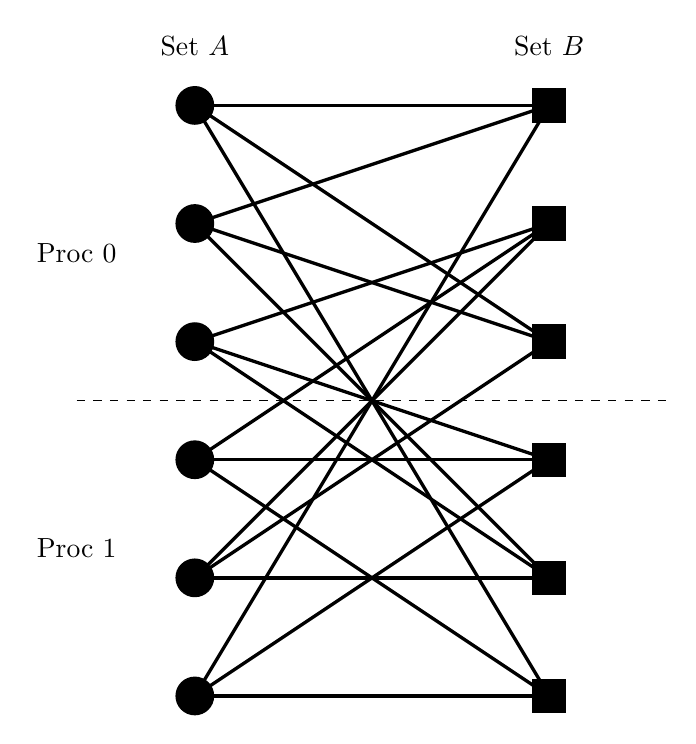
\begin{tikzpicture}[scale=1.5]


\node at (-1.5, 3) {Set $A$};
\node at (1.5, 3) {Set $B$};

\node at (-2.5, 1.25) {Proc $0$};
\node at (-2.5, -1.25) {Proc $1$};

\draw [fill=black,very thick] (-1.5,2.5) circle (0.15cm);
\draw [fill=black,very thick] (-1.5,1.5) circle (0.15cm);
\draw [fill=black,very thick] (-1.5,0.5) circle (0.15cm);
\draw [fill=black,very thick] (-1.5,-0.5) circle (0.15cm);
\draw [fill=black,very thick] (-1.5,-1.5) circle (0.15cm);
\draw [fill=black,very thick] (-1.5,-2.5) circle (0.15cm);

\draw [dashed] (-2.5,0) -- (2.5,0);

\filldraw ([xshift=-4pt,yshift=-4pt]1.5,2.5) rectangle ++(8pt,8pt);
\filldraw ([xshift=-4pt,yshift=-4pt]1.5,1.5) rectangle ++(8pt,8pt);
\filldraw ([xshift=-4pt,yshift=-4pt]1.5,0.5) rectangle ++(8pt,8pt);
\filldraw ([xshift=-4pt,yshift=-4pt]1.5,-0.5) rectangle ++(8pt,8pt);
\filldraw ([xshift=-4pt,yshift=-4pt]1.5,-1.5) rectangle ++(8pt,8pt);
\filldraw ([xshift=-4pt,yshift=-4pt]1.5,-2.5) rectangle ++(8pt,8pt);

\draw [very thick] (-1.5,2.5) -- (1.5,2.5);
\draw [very thick] (-1.5,2.5) -- (1.5,0.5);
\draw [very thick] (-1.5,2.5) -- (1.5,-2.5);

\draw [very thick] (-1.5,1.5) -- (1.5,2.5);
\draw [very thick] (-1.5,1.5) -- (1.5,0.5);
\draw [very thick] (-1.5,1.5) -- (1.5,-1.5);

\draw [very thick] (-1.5,0.5) -- (1.5,-1.5);
\draw [very thick] (-1.5,0.5) -- (1.5,-0.5);
\draw [very thick] (-1.5,0.5) -- (1.5,1.5);

\draw [very thick] (-1.5,-0.5) -- (1.5,1.5);
\draw [very thick] (-1.5,-0.5) -- (1.5,-2.5);
\draw [very thick] (-1.5,-0.5) -- (1.5,-0.5);

\draw [very thick] (-1.5,-1.5) -- (1.5,-1.5);
\draw [very thick] (-1.5,-1.5) -- (1.5,1.5);
\draw [very thick] (-1.5,-1.5) -- (1.5,0.5);

\draw [very thick] (-1.5,-2.5) -- (1.5,-0.5);
\draw [very thick] (-1.5,-2.5) -- (1.5,-2.5);
\draw [very thick] (-1.5,-2.5) -- (1.5,2.5);

\end{tikzpicture}
\caption{Data division for a random trivalent, bipartite graph.}
\end{center}
\end{figure}

%%%%%%%%%%%%% END OF PIC %%%%%%%%%%%%%%




%%%%% PROBLEMS ENCOUNTERED IN IMPLEMENTATION %%%%%


%%%%%%%%%%% DOUBLE RING PICTURE %%%%%%%%%%

\begin{figure}
\begin{center}
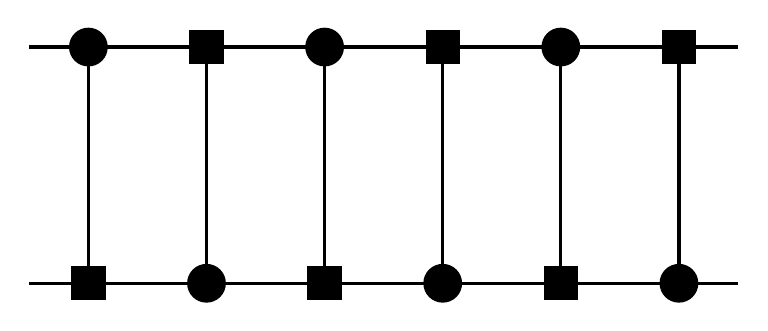
\begin{tikzpicture}[scale=1.5]

\draw [fill=black,very thick] (-2.5,1) circle (0.15cm);
\draw [fill=black,very thick] (-1.5,-1) circle (0.15cm);
\draw [fill=black,very thick] (-0.5,1) circle (0.15cm);
\draw [fill=black,very thick] (0.5,-1) circle (0.15cm);
\draw [fill=black,very thick] (1.5,1) circle (0.15cm);
\draw [fill=black,very thick] (2.5,-1) circle (0.15cm);


\filldraw ([xshift=-4pt,yshift=-4pt] -2.5,-1) rectangle ++(8pt,8pt);
\filldraw ([xshift=-4pt,yshift=-4pt] -1.5,1) rectangle ++(8pt,8pt);
\filldraw ([xshift=-4pt,yshift=-4pt] -0.5,-1) rectangle ++(8pt,8pt);
\filldraw ([xshift=-4pt,yshift=-4pt] 0.5,1) rectangle ++(8pt,8pt);
\filldraw ([xshift=-4pt,yshift=-4pt] 1.5,-1) rectangle ++(8pt,8pt);
\filldraw ([xshift=-4pt,yshift=-4pt] 2.5,1) rectangle ++(8pt,8pt);

\draw [very thick] (-3,1) -- (3,1);
\draw [very thick] (-3,-1) -- (3,-1);

\draw [very thick] (-2.5,1) -- (-2.5,-1);
\draw [very thick] (-2.5,1) -- (-1.5,1);

\draw [very thick] (-1.5,1) -- (-1.5,-1);
\draw [very thick] (-1.5,1) -- (-1.5,-1);

\draw [very thick] (-0.5,1) -- (-0.5,-1);
\draw [very thick] (-0.5,1) -- (-0.5,-1);

\draw [very thick] (0.5,1) -- (0.5,-1);
\draw [very thick] (0.5,1) -- (0.5,-1);

\draw [very thick] (1.5,1) -- (1.5,-1);
\draw [very thick] (1.5,1) -- (1.5,-1);

\draw [very thick] (2.5,1) -- (2.5,-1);
\draw [very thick] (2.5,1) -- (2.5,-1);


\end{tikzpicture}
\caption{Double ring bipartite graph.}
\end{center}
\end{figure}

%%%%%%%%% END OF PIC %%%%%%%%%%%%%%



\newpage
%%%%%%%%%%%%%%%%%%%
%%%%% RESULTS %%%%%
%%%%%%%%%%%%%%%%%%%

\section{Results}



\newpage
%%%%%%%%%%%%%%%%%%%%%%
%%%%% CONCLUSION %%%%%
%%%%%%%%%%%%%%%%%%%%%%

\section{Conclusion}

hello

\newpage
%%%%%%%%%%%%%%%%%%%%%%%
%%%%% FUTURE WORK %%%%%
%%%%%%%%%%%%%%%%%%%%%%%

\section{Future Work}
\end{document}
